\documentclass{article}
\usepackage{graphicx}
\begin{document}

\title{CS 3841 Lab 5: Let's Chat}
\author{Jeff Stubler \& Matt Edwards}
\date{24 October 2011}
\maketitle

\section*{Introduction}
We started this lab by discussing how we would design and implement it based on the given requirements. It was determined that new threads would be created to handle the UI, keyboard, time ticking, sending messages, receiving messages, and a controller thread to handle all of these. We split the work so Jeff would spend most of his time on the keyboard, time ticking, and sending and receiving of messages, while Matt would work primarily on the UI thread.

\section*{Things that went right and wrong}
Overall, this lab went well but we did not achieve the desired results. In particular, two parts of this lab went well - the server and the UI implementation. Despite this, we were not able to fully implement the lab. Due to the time constraints, being overly ambitious, and unforeseen bugs, we were not able to fully integrate the server to function with the GUI.

\section*{What we learned}
From this lab, we learned that programming sockets in C is a lot more difficult than programming sockets in Java, and protocols that are easy to use with Telnet are easier to develop. Also, we learned how to incorporate the ncurses library to create an elementary GUI with C.

\section*{Time Analysis}
In total Jeff spent about 20 hours working on this and Matt spent about 15. Most of Jeff's time was spent on the server and Matt's was divided among learning how to use ncurses and implementing the UI.

\section*{UI screenshots}

\begin{figure}[!h]
\caption{UI Implementation}
\begin{center}
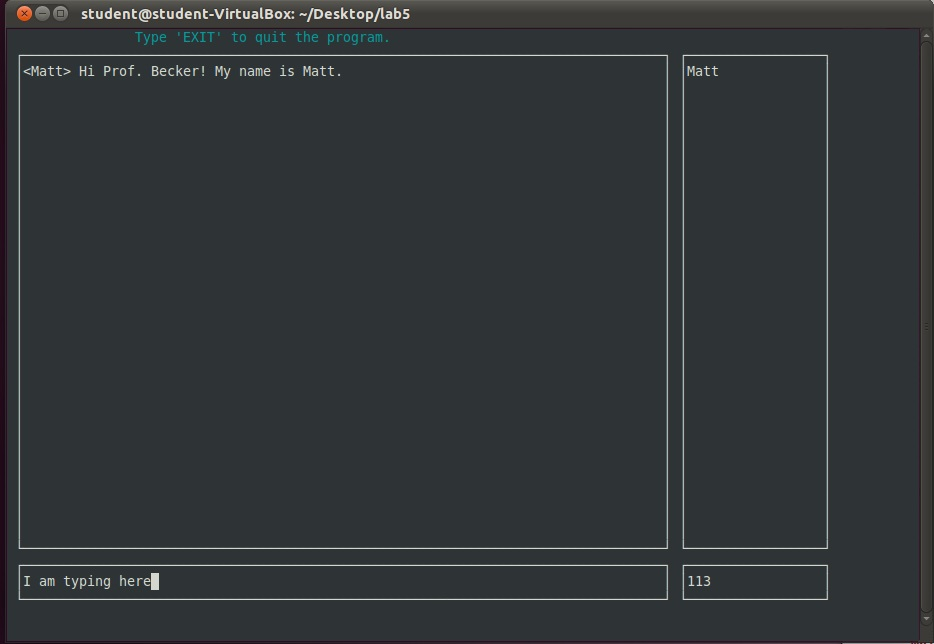
\includegraphics[scale=0.2]{ui.jpg}
\end{center}
\label{UI}
\end{figure}

\section*{Chatd screenshots}
Figures~\ref{chatd-send} and \ref{chatd-receive} show telnet sessions with the chat server, sending and receiving messages or only sending, respectively. Using telnet, the headers given with
the different message types can be seen that are normally hidden by the UI for the chat system.

\begin{figure}[!h]
\begin{center}
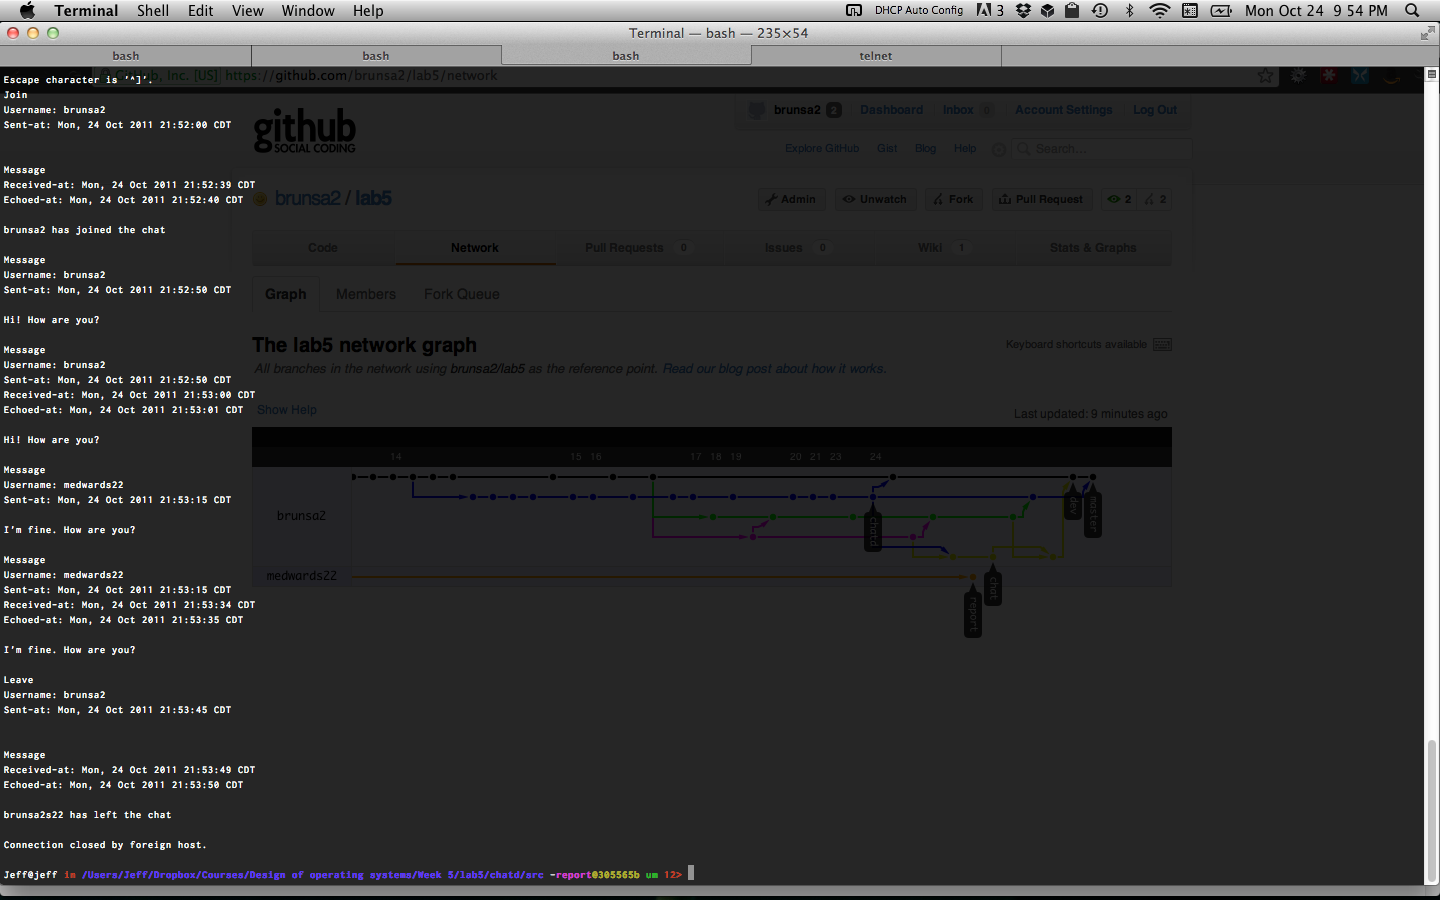
\includegraphics[scale=0.2]{send.png}
\end{center}
\caption{Telnet to chatd, sending and receiving}
\label{chatd-send}
\end{figure}

\begin{figure}[!h]
\begin{center}
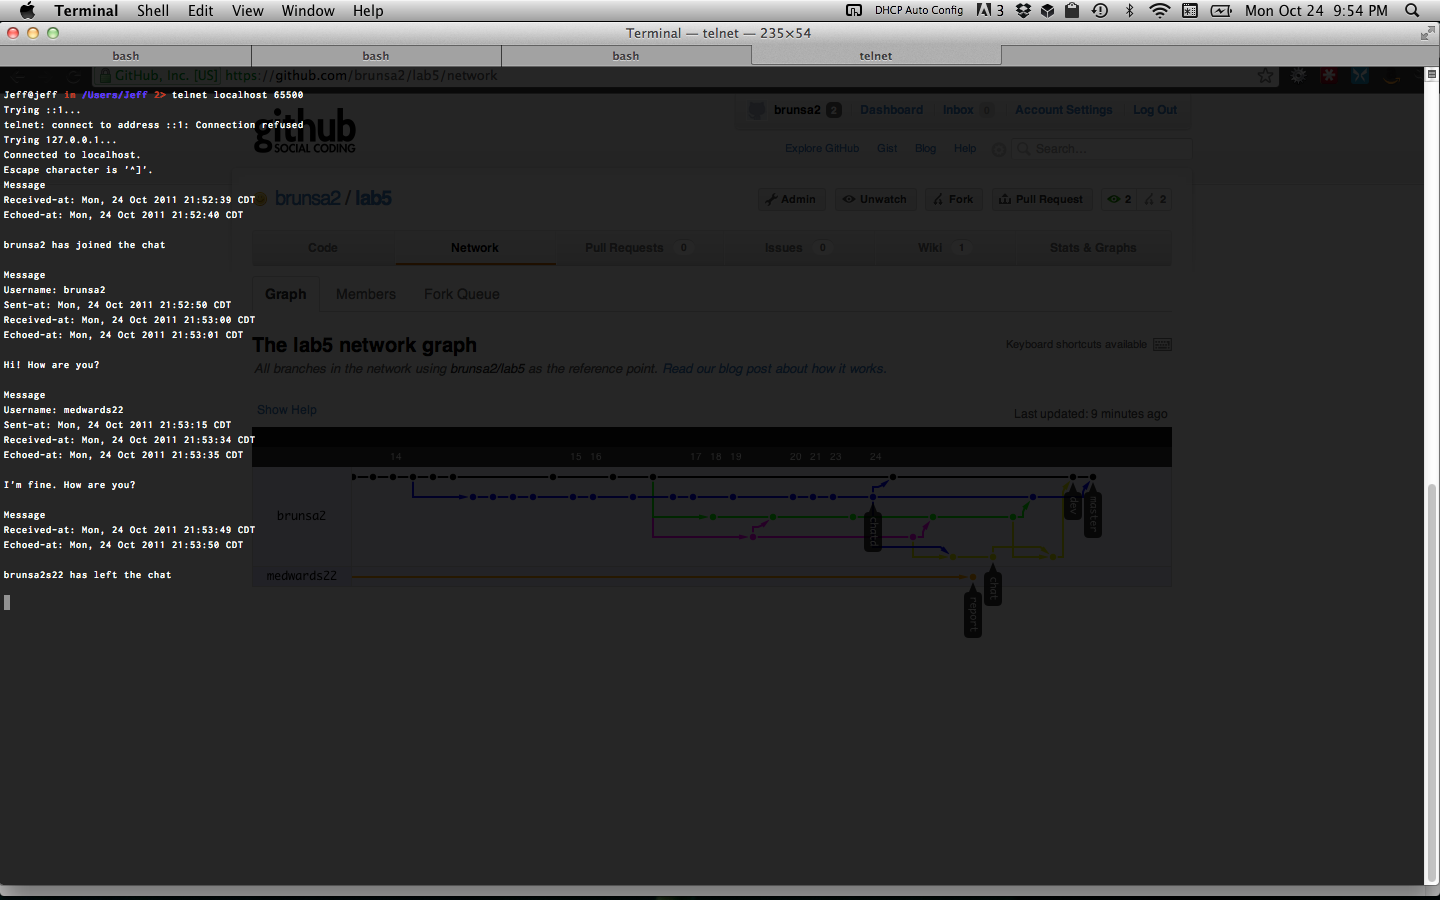
\includegraphics[scale=0.2]{receive.png}
\end{center}
\caption{Telnet to chatd, sending only}
\label{chatd-receive}
\end{figure}

\section*{Conclusion}
In this lab, we constructed code using POSIX threads, protected against race conditions, communicated using sockets, and implemented a GUI with ncurses. We learned quite a bit from this lab and spent a decent amount of time making trying to implement all desired functionality.

\section*{Appendix: Source code}

\subsection*{controller.c}

\begin{verbatim}

/*
 * Jeff Stubler
 * CS 3841
 * Lab 5 -- UNIX chat program
 * 14 October 2011
 *
 * Main controller thread
 */

#include "controller.h"

void ctrl_thread(void) {
    int x = 0;
    for(x = 0; x < 5; x++) {
        sleep(10);
        printf("Alive\n");
    }
}

void clock_tick(void) {
    
}

void string_entered(void) {
    
}

void network_ready(void) {
    
}

void message_arrived(void) {
    
}

\end{verbatim}

\subsection*{controller.h}

\begin{verbatim}

/*
 * Jeff Stubler
 * CS 3841
 * Lab 5 -- UNIX chat program
 * 14 October 2011
 *
 * Main controller thread
 */

#ifndef CONTROLLER
#define CONTROLLER

#include <stdio.h>

#include "tick.h"
#include "keyboard.h"

void ctrl_thread(void);
void clock_tick(void);
void string_entered(void);
void network_ready(void);
void message_arrived(void);

#endif

\end{verbatim}

\subsection*{keyboard.c}

\begin{verbatim}

/*
 * Jeff Stubler
 * CS 3841
 * Lab 5 -- UNIX chat program
 * 13 October 2011
 *
 * Keyboard buffer system
 */

#include "keyboard.h"

#define KB_BUFFER_SIZE 16
#define KB_FIRST_TAIL 0
#define KB_FIRST_HEAD 1

#define adjusted_head(head) (head == 0 ? 16 : head)

//extern ncurses_initialized;
mutex_id kb_buffer_mutex = PTHREAD_MUTEX_INITIALIZER;

static char kb_buffer[KB_BUFFER_SIZE];
static int kb_buffer_head = KB_FIRST_HEAD, kb_buffer_tail = KB_FIRST_TAIL;

void *kb_thread(void *argument) {
    char next_character;
    //while(!ncurses_initialized);
    while(true) {
        next_character = getchar();
        lock(&kb_buffer_mutex);
        while(kb_buffer_head == kb_buffer_tail);
        kb_buffer[kb_buffer_head] = next_character;
        kb_buffer_head = (kb_buffer_head + 1) % KB_BUFFER_SIZE;
        unlock(&kb_buffer_mutex);
    }
    
    return NULL;
}

bool kb_has_key(void) {
    lock(&kb_buffer_mutex);
    if(adjusted_head(kb_buffer_head) - kb_buffer_tail == 1) {
        unlock(&kb_buffer_mutex);
        return false;
    } else {
        unlock(&kb_buffer_mutex);
        return true;
    }
}

char kb_get_key(void) {
    char next_key;
    lock(&kb_buffer_mutex);
    if(!kb_has_key()) {
        unlock(&kb_buffer_mutex);
        return '\0';
    } else {
        next_key = kb_buffer[kb_buffer_tail];
        kb_buffer_tail = (kb_buffer_head + 1) & KB_BUFFER_SIZE;
        unlock(&kb_buffer_mutex);
        return next_key;
    }
}

\end{verbatim}

\subsection*{keyboard.h}

\begin{verbatim}

/*
 * Jeff Stubler
 * CS 3841
 * Lab 5 -- UNIX chat program
 * 13 October 2011
 *
 * Keyboard buffer system
 */

#ifndef KEYBOARD
#define KEYBOARD

#include <stdio.h>
#include <stdbool.h>
#include <pthread.h>

#include "thread.h"

void *kb_thread(void *);
bool kb_has_key(void);
char kb_get_key(void);

#endif

\end{verbatim}

\subsection*{main.c}

\begin{verbatim}

/*
 * Jeff Stubler
 * CS 3841
 * Lab 5 -- UNIX chat program
 * 12 October 2011
 *
 * Main entry point for client, gathers arguments, starts threads, and acts as
 * main controller for system
 */

#include "main.h"

#define fatal_shutdown(message) fprintf(stderr, "%s\n", message); \
        exit(EXIT_FAILURE);

/* Variables for parsing command line arguments */
extern int optind, opterr, optopt;
extern char *optarg;
extern int network_error_code;

login_info login;

static void print_usage_and_exit_with_code(int exit_status) {
    fprintf(stderr, "Usage: chat [OPTION]... host\n"
            "Talk among other users connected to a chat server.\n\n"
            /*"-a\t\tJoin anonymously without greeting message\n"*/
            "-h, --help\tDisplay this help and exit\n"
            "-p\t\tSpecify port to connect to server on\n"
            "-u\t\tSet username to be displayed to chat members\n\n");
    exit(exit_status);
}

int main(int argc, char **argv) {
    int option, thread_error_code;
    thread_id kb_thread_id, tick_thread_id, ui_thread_id, network_thread_id;
    void *return_value;
    
    if(argc > 1 && strcmp(argv[1], "--help") == 0) {
        print_usage_and_exit_with_code(EXIT_SUCCESS);
    }
    
    while((option = getopt(argc, argv, ":ahp:u:")) != -1) {        
        switch(option) {
            case 'a':
                login.anonymous = true;
            case 'h':
                print_usage_and_exit_with_code(EXIT_SUCCESS);
            case 'p':
                if(login.port != NULL) {
                    free(login.port);
                }
                login.port = (char *) malloc(strlen(optarg));
                strcpy(login.port, optarg);
                break;
            case 'u':
                if(login.username != NULL) {
                    free(login.username);
                }
                login.username = (char *) malloc(strlen(optarg));
                strcpy(login.username, optarg);
                break;
            case ':':
                fprintf(stderr, "Missing argument for %c option\n\n", optopt);
                print_usage_and_exit_with_code(EXIT_FAILURE);
            case '?':
                fprintf(stderr, "Unrecognized flag %c\n\n", optopt);
                print_usage_and_exit_with_code(EXIT_FAILURE);
            default:
                fatal_shutdown("Unexpected response from option parser");
        }
    }
    
    if(optind < argc) {
        login.server = (char *) malloc(strlen(argv[optind]));
        strcpy(login.server, argv[optind]);
    } else {
        fprintf(stderr, "Missing host name\n\n");
        print_usage_and_exit_with_code(EXIT_FAILURE);
    }
    
    /* TODO: Check for null for any login block information and set it to a
     * default value */
    
    start_thread(&kb_thread_id, kb_thread, NULL);
    start_thread(&tick_thread_id, tick_thread, NULL);
    start_thread(&ui_thread_id, ui_thread, NULL);
    printf("Connecting...\n");
    start_thread(&network_thread_id, network_thread, NULL);
    
    sleep(2);
    if(network_error_code != 0) {
        printf("Could not connect\nError code %d\n", network_error_code);
        exit(EXIT_FAILURE);
    }
    
    ctrl_thread();
    
    free(login.username);
    free(login.server);
    free(login.port);
    
    return 0;
}

\end{verbatim}

\subsection*{network.c}

\begin{verbatim}

/*
 * Jeff Stubler
 * CS 3841
 * Lab 5 -- UNIX chat program
 * 14 October 2011
 *
 * Network startup thread
 */

#include "network.h"

extern login_info login;
int network_error_code;
int sock_fd;

void *network_thread(void *argument) {
    thread_id send_thread_id, receive_thread_id;
    struct addrinfo hints, *servinfo, *current_addr;
    int gai_error_code;
    
    memset(&hints, 0, sizeof(hints));
    hints.ai_family = AF_UNSPEC;
    hints.ai_socktype = SOCK_STREAM;
    
    if((gai_error_code = getaddrinfo(login.server, login.port, &hints, &servinfo)) != 0) {
        network_error_code = -1;
        return NULL;
    }
    
    for(current_addr = servinfo; current_addr != NULL; current_addr =       
            current_addr->ai_next) {
        if((sock_fd = socket(current_addr->ai_family,
                              current_addr->ai_socktype, current_addr->ai_protocol)) == -1) {
            continue;
        }
        
        if(connect(sock_fd, current_addr->ai_addr, current_addr->ai_addrlen) == -1) {
            close(sock_fd);
            continue;
        }
        
        break;
    }
    
    if(current_addr == NULL) {
        network_error_code = -1;
        return NULL;
    }
    
    freeaddrinfo(servinfo);
    
    network_ready();
    
    write(sock_fd,
          "Join\r\rUsername: brunsa2\r\n\r\n\r\n",
          strlen("Join\r\rUsername: brunsa2\r\n\r\n\r\n"));
    write(sock_fd,
          "Message\r\nUsername: brunsa2\r\n\r\nHi! How are you?\r\n\r\n",
          strlen("Message\r\nUsername: brunsa2\r\n\r\nHi! How are you?\r\n\r\n"));
    
    //start_joinable_thread(&send_thread_id, send_thread, &sock_fd);
    start_joinable_thread(&receive_thread_id, receive_thread, &sock_fd);
    
    join_thread(&send_thread_id);
    join_thread(&receive_thread_id);
    
    close(sock_fd);
    
    return NULL;
}

\end{verbatim}

\subsection*{network.h}

\begin{verbatim}

/*
 * Jeff Stubler
 * CS 3841
 * Lab 5 -- UNIX chat program
 * 14 October 2011
 *
 * Network startup thread
 */

#ifndef NETWORK
#define NETWORK

#include <stdio.h>
#include <syslog.h>
#include <stdbool.h>
#include <stdlib.h>
#include <unistd.h>
#include <string.h>
#include <errno.h>
#include <sys/types.h>
#include <sys/socket.h>
#include <netinet/in.h>
#include <netdb.h>
#include <arpa/inet.h>
#include <sys/wait.h>

#include "thread.h"
#include "main.h"

typedef struct {
    char *username;
    char *message_text;
} message;

#include "send.h"
#include "receive.h"

void *network_thread(void *);

#endif

\end{verbatim}

\subsection*{receive.c}

\begin{verbatim}

/*
 * Jeff Stubler
 * CS 3841
 * Lab 5 -- UNIX chat program
 * 14 October 2011
 *
 * Network receive thread
 */

#include "receive.h"

void *receive_thread(void *argument) {
    return NULL;
}

message *get_message(void) {
    return NULL;
}

\end{verbatim}

\subsection*{receive.h}

\begin{verbatim}

/*
 * Jeff Stubler
 * CS 3841
 * Lab 5 -- UNIX chat program
 * 14 October 2011
 *
 * Network receive thread
 */

#ifndef NETWORK_RECEIVE
#define NETWORK_RECEIVE

#include <stdlib.h>

#include "network.h"

void *receive_thread(void *);
message *get_message(void);

#endif

\end{verbatim}

\subsection*{send.c}

\begin{verbatim}

/*
 * Jeff Stubler
 * CS 3841
 * Lab 5 -- UNIX chat program
 * 14 October 2011
 *
 * Network send thread
 */

#include "send.h"

void *send_thread(void *argument) {
    int sock_fd = (int) ((void *) argument);
    
    write(sock_fd,
          "Join\r\rUsername: brunsa2\r\n\r\n\r\n",
          strlen("Join\r\rUsername: brunsa2\r\n\r\n\r\n"));
    write(sock_fd,
          "Message\r\nUsername: brunsa2\r\n\r\nHi! How are you?\r\n\r\n",
          strlen("Message\r\nUsername: brunsa2\r\n\r\nHi! How are you?\r\n\r\n"));
    
    return NULL;
}

void send_message(message *sending_message) {
    
}

\end{verbatim}

\subsection*{send.h}

\begin{verbatim}

/*
 * Jeff Stubler
 * CS 3841
 * Lab 5 -- UNIX chat program
 * 14 October 2011
 *
 * Network send thread
 */

#ifndef NETWORK_SEND
#define NETWORK_SEND

#include <stdlib.h>

#include "network.h"

void *send_thread(void *);
void send_message(message *);

#endif

\end{verbatim}

\subsection*{thread.c}

\begin{verbatim}

/*
 * Jeff Stubler
 * CS 3841
 * Lab 5 -- UNIX chat program
 * 12 October 2011
 *
 * Thread convenience functions, wraps around Pthreads
 */

#include "thread.h"

#define fatal_shutdown(message) fprintf(stderr, "%s\n", message); \
exit(EXIT_FAILURE);

/* TODO: Look further at thread priority */

void start_thread(pthread_t *thread, void *(* thread_function)(void *),
                  void *argument) {
    int thread_error_code;
    pthread_attr_t attributes;
    
    thread_error_code = pthread_attr_init(&attributes);
    if(thread_error_code != 0) {
        fatal_shutdown("Error initializing thread attributes");
    }
    
    thread_error_code = pthread_attr_setdetachstate(&attributes,
                                                    PTHREAD_CREATE_DETACHED);
    if(thread_error_code != 0) {
        fatal_shutdown("Error setting thread detach state attribute");
    }
    
    thread_error_code = pthread_create(thread, &attributes, thread_function,
                                       argument);
    if(thread_error_code != 0) {
        fatal_shutdown("Error starting thread");
    }
    
    thread_error_code = pthread_attr_destroy(&attributes);
    if(thread_error_code != 0) {
        fatal_shutdown("Error destroying attributes");
    }
}

void start_joinable_thread(pthread_t *thread, void *(* thread_function)(void *),
                           void *argument) {
    int thread_error_code;
    
    thread_error_code = pthread_create(thread, NULL, thread_function, argument);
    if(thread_error_code != 0) {
        fatal_shutdown("Error starting thread");
    }
}

void join_thread(pthread_t *thread) {
    pthread_t joined_thread;
    memcpy(&joined_thread, thread, sizeof(thread));
    pthread_join(joined_thread, NULL);
}

void initialize_mutex(mutex_id *mutex) {
    int mutex_error_code;
    mutex_error_code = pthread_mutex_init(mutex, NULL);
    if(mutex_error_code != 0) {
        fatal_shutdown("Error initializing mutex");
    }
}

void lock(mutex_id *mutex) {
    pthread_mutex_lock(mutex);
}

void unlock(mutex_id *mutex) {
    pthread_mutex_unlock(mutex);
}

void destroy_mutex(mutex_id *mutex) {
    int mutex_error_code;
    unlock(mutex);
    mutex_error_code = pthread_mutex_destroy(mutex);
    if(mutex_error_code != 0) {
        fatal_shutdown("Error destroying mutex");
    }
}

\end{verbatim}

\subsection*{thread.h}

\begin{verbatim}

/*
 * Jeff Stubler
 * CS 3841
 * Lab 5 -- UNIX chat program
 * 12 October 2011
 *
 * Thread convenience functions, wraps around Pthreads
 */

#ifndef THREADS
#define THREADS

#include <pthread.h>
#include <stdio.h>
#include <stdlib.h>
#include <string.h>

typedef pthread_t thread_id;
typedef pthread_mutex_t mutex_id;

void start_thread(pthread_t *, void *(* thread_function)(void *), void *);
void start_joinable_thread(pthread_t *, void *(* thread_function)(void *),
                           void *);
void join_thread(pthread_t *);
void initialize_mutex(mutex_id *);
void lock(mutex_id *);
void unlock(mutex_id *);
void destroy_mutex(mutex_id *);

#endif

\end{verbatim}

\subsection*{tick.c}

\begin{verbatim}

/*
 * Jeff Stubler
 * CS 3841
 * Lab 5 -- UNIX chat program
 * 14 October 2011
 *
 * Tick counting thread
 */

#include "tick.h"

#define MICROSECONDS_BETWEEN_CLOCK_UPDATE 1000000

static start_ticks, elapsed_ticks;

void *tick_thread(void *argument) {
    start_ticks = time(NULL);
    
    while(true) {
        elapsed_ticks = time(NULL) - start_ticks;
        usleep(MICROSECONDS_BETWEEN_CLOCK_UPDATE);
        clock_tick();
    }
    
    return NULL;
}

int get_elapsed_ticks(void) {
    return elapsed_ticks;
}

\end{verbatim}

\subsection*{tick.h}

\begin{verbatim}

/*
 * Jeff Stubler
 * CS 3841
 * Lab 5 -- UNIX chat program
 * 14 October 2011
 *
 * Tick counting thread
 */

#ifndef TICK
#define TICK

#include <stdio.h>
#include <time.h>
#include <stdbool.h>

#include "controller.h"

void *tick_thread(void *);
int get_elapsed_ticks(void);

#endif

\end{verbatim}

\subsection*{daemon.c}

\begin{verbatim}

/*
 * Jeff Stubler
 * CS 3841
 * Lab 5 -- UNIX chat program
 * 12 October 2011
 *
 * Daemonizing function to start server running
 */

#include "daemon.h"

#define PID_STRING_LENGTH 16

#define fatal_shutdown(message) syslog(LOG_CRIT, message); \
        exit(EXIT_FAILURE);
#define nonfatal_shutdown(message) syslog(LOG_NOTICE, message); \
        exit(EXIT_SUCCESS);

int become_daemon(void (* sig_handler)(int)) {
    struct sigaction sigact;
    int maximum_fd, current_fd, lock_fd;
    char pid_string[PID_STRING_LENGTH];
    
    openlog("chatd", LOG_CONS, LOG_USER);
    
    syslog(LOG_INFO, "This is chatd. 14 October 2011 Jeff Stubler for CS 3841 "
            "UNIX chat system lab 5");
    
    sigemptyset(&sigact.sa_mask);
    sigact.sa_flags = SA_RESTART;
    sigact.sa_handler = sig_handler;
    if(sigaction(SIGHUP, &sigact, NULL) == -1) {
        fatal_shutdown("Error setting SIGHUP signal handler");
    }
    if(sigaction(SIGTERM, &sigact, NULL) == -1) {
        fatal_shutdown("Error setting SIGTERM signal handler");
    }
    if(signal(SIGPIPE, SIG_IGN) == SIG_ERR) {
        fatal_shutdown("Error ignoring SIGPIPE signal");
    }
    
    /* Become a background process */
    switch(fork()) {
        case -1:
            fatal_shutdown("Error becomming background process");
        case 0:
            /* Child process should continue */
            break;
        default:
            _exit(EXIT_SUCCESS);
    }
    
    /* Become leader of new session */
    if(setsid() == -1) {
        fatal_shutdown("Error becomming session leader");
    }
    
    /* Ensure that we are not leader of new session */
    switch(fork()) {
        case -1:
            fatal_shutdown("Error breaking from leadership of new session");
        case 0:
            /* Child process should continue */
            break;
        default:
            _exit(EXIT_SUCCESS);
    }
    
    syslog(LOG_INFO, "chatd is now running in the background");
    
    /* Clear file mode creation mask and chdir to root */
    umask(0027);
    //chdir("/");
    
    /* Close all files */
    maximum_fd = sysconf(_SC_OPEN_MAX);
    if(maximum_fd == -1) {
        maximum_fd = MAX_FILE_DESCRIPTOR_TO_CLOSE;
    }
    for(current_fd = 0; current_fd < maximum_fd; current_fd++) {
        close(current_fd);
    }
    
    /* std*** to /dev/null */
    close(STDIN_FILENO);
    
    current_fd = open("/dev/null", O_RDWR);
    
    if(current_fd != STDIN_FILENO) {
        fatal_shutdown("Cannot attach stdin to /dev/null");
    }
    if(dup2(STDIN_FILENO, STDOUT_FILENO) != STDOUT_FILENO) {
        fatal_shutdown("Cannot attach stdout to /dev/null");
    }
    if(dup2(STDIN_FILENO, STDERR_FILENO) != STDERR_FILENO) {
        fatal_shutdown("Cannot attach stderr to /dev/null");
    }
    
    syslog(LOG_INFO, "chatd is ready to lock system");
    
    /* Create lock file */
    lock_fd = open("chatd.lock", O_RDWR | O_CREAT, 0640);
    if(lock_fd < 0) {
        fatal_shutdown("Cannot open lock file");
    }
    if(lockf(lock_fd, F_TLOCK, 0) < 0) {
        nonfatal_shutdown("chatd is already running---this chatd will stop");
    }
    
    sprintf(pid_string, "%d\n", getpid());
    write(lock_fd, pid_string, strlen(pid_string));
    
    syslog(LOG_INFO, "chatd is locked");
    syslog(LOG_INFO, "chatd has started successfully");
    
    return 0;
}

\end{verbatim}

\subsection*{daemon.h}

\begin{verbatim}

/*
 * Jeff Stubler
 * CS 3841
 * Lab 5 -- UNIX chat program
 * 12 October 2011
 *
 * Daemonizing function to start server running
 */

#ifndef DAEMON
#define DAEMON

#include <sys/stat.h>
#include <stdlib.h>
#include <unistd.h>
#include <fcntl.h>
#include <stdio.h>
#include <string.h>
#include <syslog.h>
#include <signal.h>

#define MAX_FILE_DESCRIPTOR_TO_CLOSE 8192

int become_daemon(void (* sig_handler)(int)); 

#endif

\end{verbatim}

\subsection*{chatd.c}

\begin{verbatim}

/*
 * Jeff Stubler
 * CS 3841
 * Lab 5 -- UNIX chat program
 * 12 October 2011
 *
 * Daemon process that receives message and redistributes it to all connected
 * chat clients
 */

#include "chatd.h"

#define READ_BUFFER_SIZE 1024
#define MAX_TOKEN_SIZE 1024
#define PORT_STR_LENGTH 8

#define fatal_shutdown(message) fprintf(stderr, "%s\n", message); \
        exit(EXIT_FAILURE);

typedef struct {
    int port;
    int max_threads;
    int send_time, send_time_idle, send_time_idle_after;
    int shutdown_delay;
    bool send_join_messages, send_leave_messages;
    bool shutdown_cancel;
} configuration;

static void init_configuration(configuration *config) {
    config->port = 65500;
    config->max_threads = 32;
    config->send_time = 600;
    config->send_time_idle = 900;
    config->send_time_idle_after = 600;
    config->shutdown_delay = 120;
    config->send_join_messages = true;
    config->send_leave_messages = true;
    config->shutdown_cancel = true;
}

configuration config;
bool should_terminate;

int sock_fd;
struct linkedList thread_list;

static void parse_configuration_line(configuration *config,
        char *configuration_line) {
    char identifier_token[MAX_TOKEN_SIZE];
    int value_token;
    
    if(sscanf(configuration_line, "%1023s %d", identifier_token,
            &value_token) < 2) {
        return;
    }
    
    if(strcmp(identifier_token, "port") == 0) {
        config->port = value_token;
    }
    
    if(strcmp(identifier_token, "max-threads") == 0) {
        config->max_threads = value_token;
    }
    
    if(strcmp(identifier_token, "send-time") == 0) {
        config->send_time = value_token;
    }
    
    if(strcmp(identifier_token, "send-time-idle") == 0) {
        config->send_time_idle = value_token;
    }
    
    if(strcmp(identifier_token, "send-time-idle-after") == 0) {
        config->send_time_idle_after = value_token;
    }
    
    if(strcmp(identifier_token, "send-join-messages") == 0) {
        config->send_join_messages = value_token == 1;
    }
    
    if(strcmp(identifier_token, "send-leave-messages") == 0) {
        config->send_leave_messages = value_token == 1;
    }
    
    if(strcmp(identifier_token, "shutdown-delay") == 0) {
        config->shutdown_delay = value_token;
    }
    
    if(strcmp(identifier_token, "shutdown-cancel") == 0) {
        config->shutdown_cancel = value_token == 1;
    }
}

static void read_configuration(configuration *config) {
    FILE *conf_fd;
    char conf_line[READ_BUFFER_SIZE];
    
    /* TODO: Check if file has right permissions */
    
    conf_fd = fopen("/etc/chat.conf", "r");
    if(conf_fd == NULL) {
        fatal_shutdown("Could not open configuration file");
    }
    
    while(fgets(conf_line, READ_BUFFER_SIZE, conf_fd) != NULL) {
        parse_configuration_line(config, conf_line);
    }
    
    if(fclose(conf_fd) != 0) {
        fatal_shutdown("Could not close configuration file");
    }
    
    syslog(LOG_DEBUG, "Port: %d. Max Threads: %d", config->port,
            config->max_threads);
    syslog(LOG_DEBUG, "Send time: %d unless no message in %d then %d",
            config->send_time, config->send_time_idle_after,
            config->send_time_idle);
    syslog(LOG_DEBUG, "Shutdown delay: %d", config->shutdown_delay);
    if(config->send_join_messages) {
        syslog(LOG_DEBUG, "Send join messages");
    }
    if(config->send_leave_messages) {
        syslog(LOG_DEBUG, "Send leave messages");
    }
    if(config->shutdown_cancel) {
        syslog(LOG_DEBUG, "Shutdown cancel enabled");
    }
}

static void chatd() {
    struct addrinfo hints, *servinfo, *current_addr;
    char port_str[PORT_STR_LENGTH];
    int gai_error_code;
    int yes = 1;
    int thread_index;
    thread_data new_thread;
    
    init_configuration(&config);
    read_configuration(&config);
    
    memset(&hints, 0, sizeof(hints));
    hints.ai_socktype = SOCK_STREAM;
    hints.ai_flags = AI_PASSIVE;
    
    sprintf(port_str, "%d", config.port);
    
    if((gai_error_code = getaddrinfo(NULL, port_str, &hints, &servinfo)) != 0) {
        syslog(LOG_CRIT, "Could not get address info: %s",
                gai_strerror(gai_error_code));
        exit(EXIT_FAILURE);
    }
    
    for(current_addr = servinfo; current_addr != NULL;
            current_addr = current_addr->ai_next) {
        if((sock_fd = socket(current_addr->ai_family, current_addr->ai_socktype,
                current_addr->ai_protocol)) == -1) {
            syslog(LOG_INFO, "Could not open socket with this address");
            continue;
        }
        
        if(setsockopt(sock_fd, SOL_SOCKET, SO_REUSEADDR, &yes,
                      sizeof(int)) == -1) {
            syslog(LOG_INFO, "Could not set up reusable addresses");
            exit(EXIT_FAILURE);
        }
        
        if(bind(sock_fd, current_addr->ai_addr, current_addr->ai_addrlen) ==
                -1) {
            close(sock_fd);
            syslog(LOG_INFO, "Could not bind to socket with this address");
            continue;
        }
        
        break;
    }
    
    if(current_addr == NULL) {
        syslog(LOG_CRIT, "Could not bind to socket");
        exit(EXIT_FAILURE);
    }
    
    freeaddrinfo(servinfo);
    
    if(listen(sock_fd, config.max_threads) == -1) {
        syslog(LOG_CRIT, "Could not listen");
        exit(EXIT_FAILURE);
    }
    
    ll_init(&thread_list);
    
    syslog(LOG_INFO, "Using socket fd %d", sock_fd);
    
    for(thread_index = 0; thread_index < config.max_threads; thread_index++) {
        thread_id thread;
        memset(&new_thread, 0, sizeof(new_thread));
        new_thread.socket = sock_fd;
        new_thread.should_shutdown = 0;
        new_thread.message_queue =
                (struct linkedList *) malloc(sizeof(struct linkedList));
        ll_init(new_thread.message_queue);
        ll_add(&thread_list, &new_thread, sizeof(new_thread));
        syslog(LOG_INFO, "Initialized thread %d", thread_index);
        start_thread(&thread, socket_thread,
                ll_get(&thread_list, thread_index));
    }
    
    for(;;) {
        sleep(10);
    }
}

void dispatch_message(message *dispatched_message) {
    struct linkedListIterator *iterator;
    iterator = ll_getIterator(&thread_list);
    while(ll_hasNext(iterator)) {
        thread_data *thread = ll_next(iterator);
        message *new_message;
        int line_index;
        
        new_message = (message *) malloc(sizeof(message));
        if(new_message == NULL) {
            continue;
        }
        new_message->header_size = dispatched_message->header_size;
        new_message->message_size = dispatched_message->message_size;
        new_message->headers = (char **) malloc(MAX_HEADERS * sizeof(char *));
        new_message->message = (char **) malloc(MAX_MESSAGES * sizeof(char *));
        
        for(line_index = 0; line_index < dispatched_message->header_size; line_index++) {
            new_message->headers[line_index] = (char *) malloc(strlen(dispatched_message->headers[line_index]));
            strcpy(new_message->headers[line_index], dispatched_message->headers[line_index]);
        }
        for(line_index = 0; line_index < dispatched_message->message_size; line_index++) {
            new_message->message[line_index] = (char *) malloc(strlen(dispatched_message->message[line_index]));
            strcpy(new_message->message[line_index], dispatched_message->message[line_index]);
        }
        
        ll_add(thread->message_queue, new_message, sizeof(message));
        
        free(new_message);
    }
    free(iterator);
}

void signal_handler(int signal) {
    switch(signal) {
        case SIGHUP:
            syslog(LOG_INFO, "chatd is refreshing");
            read_configuration(&config);
            break;
        case SIGTERM:
            should_terminate = true;
            syslog(LOG_INFO, "chatd is stopping");
            close(sock_fd);
            syslog(LOG_INFO, "chatd has stopped");
            exit(EXIT_SUCCESS);
    }
}

int main(int argc, char **argv) {
    become_daemon(signal_handler);
    chatd();
    return 0;
}

\end{verbatim}

\subsection*{chatd.h}

\begin{verbatim}

/*
 * Jeff Stubler
 * CS 3841
 * Lab 5 -- UNIX chat program
 * 12 October 2011
 *
 * Definitions and prototypes for chat daemon
 */

#ifndef CHATD
#define CHATD

#define MAX_HEADERS 16
#define MAX_MESSAGES 4

#include <stdio.h>
#include <syslog.h>
#include <stdbool.h>
#include <stdlib.h>
#include <unistd.h>
#include <string.h>
#include <errno.h>
#include <sys/types.h>
#include <sys/socket.h>
#include <netinet/in.h>
#include <netdb.h>
#include <arpa/inet.h>
#include <sys/wait.h>

#include "daemon.h"
#include "linkedlist.h"
#include "thread.h"

typedef struct {
    int socket;
    struct linkedList *message_queue;
    int should_shutdown;
} thread_data;

typedef struct {
    char **headers;
    int header_size;
    char **message;
    int message_size;
} message;

#include "socketthread.h"

void signal_handler(int);
void dispatch_message(message *);

#endif

\end{verbatim}

\subsection*{linkedlist.c}

\begin{verbatim}

/*
 * Jeff Stubler
 * CS 3841
 * A Linked List in C
 * 21 September 2011
 *
 * Defines implementations of functions needed to initialize, modify, and
 * traverse a doubly-linked list.
 */

#include <stdbool.h>
#include <string.h>
#include <stdint.h>
#include <stdlib.h>
#include "linkedlist.h"

/* Initialize linked list structure
  *
  * Takes: pointer to linked list
  * Gives: initialized empty linked list
 */
void ll_init(struct linkedList *linked_list) {
    if(!linked_list) {
        return;
    }
    
    linked_list->head = NULL;
    linked_list->tail = NULL;
    linked_list->size = 0;
}

/* Clears linked list structure including freeing memory
  *
  * Takes: pointer to linked list
  * Gives: cleared linked list and freed memory
 */
void ll_clear(struct linkedList *linked_list) {
    if(!(linked_list && linked_list->head && linked_list->tail)) {
        return;
    }
    
    struct listNode *current = linked_list->tail;
    while(current->next) {
        free(current->data);
        current = current->next;
        free(current->previous);
    }
    free(current->data);
    free(current);
    linked_list->head = NULL;
    linked_list->tail = NULL;
    linked_list->size = 0;
}

/* Adds data of specified size to end of linked list
  *
  * Takes: pointer to linked list, pointer to data, and size of data in bytes
  * Gives: true if success, false if failure
 */
bool ll_add(struct linkedList *linked_list, void *object, int size) {
    struct listNode *new_node;
    
    if(!(linked_list && object)) {
        return false;
    }
    
    new_node = (struct listNode *) malloc(sizeof(struct listNode));
    if(new_node == NULL) {
        return false;
    }
    
    new_node->data = (void *) malloc(size);
    if(new_node->data == NULL) {
        free(new_node);
        return false;
    }
    
    memcpy(new_node->data, object, size);
    new_node->dataSize = size;
    new_node->next = NULL;
    new_node->previous = linked_list->tail;
    if(linked_list->tail) {
        linked_list->tail->next = new_node;
    }
    if(!linked_list->head) {
        linked_list->head = new_node;
    }
    linked_list->tail = new_node;
    linked_list->size++;
    
    return true;
}

/* Adds data of specified size to specified position in linked list (index is position where new item appears)
 *
 * Takes: pointer to linked list, pointer to data, size of data in bytes, index of item in list
 * Gives: true if success, false if failure
 */

bool ll_addIndex(struct linkedList *linked_list, void *object, int size, int index) {
    int traversingIndex;
    struct listNode *node_after_new_node, *new_node;
    
    if(!(linked_list && object && index >= 0 && index < ll_size(linked_list))) {
        return false;
    }
    
    node_after_new_node = linked_list->head;
    for(traversingIndex = 0; traversingIndex < index; traversingIndex++) {
        node_after_new_node = node_after_new_node->next;
    }
    
    new_node = (struct listNode *) malloc(sizeof(struct listNode));
    if(new_node == NULL) {
        return false;
    }
    
    new_node->data = (void *) malloc(size);
    if(new_node->data == NULL) {
        free(new_node);
        return false;
    }
    
    memcpy(new_node->data, object, size);
    new_node->dataSize = size;
    new_node->previous = node_after_new_node->previous;
    new_node->next = node_after_new_node;
    if(node_after_new_node->previous) {
        node_after_new_node->previous->next = new_node;
    }
    node_after_new_node->previous = new_node;
    if(index == 0) {
        linked_list->head = new_node;
    }
    linked_list->size++;
    
    return true;
}

/* Removes the list item at given index
 *
 * Takes: pointer to linked list, index to remove
 * Gives: true if successful, false otherwise
 */

bool ll_remove(struct linkedList *linked_list, int index) {
    int traversingIndex;
    struct listNode *node_to_delete;
    
    if(!(linked_list && index >= 0 && index < ll_size(linked_list))) {
        return false;
    }
    
    node_to_delete = linked_list->head;
    for(traversingIndex = 0; traversingIndex < index; traversingIndex++) {
        node_to_delete = node_to_delete->next;
    }
    
    if(node_to_delete->next) {
        node_to_delete->next->previous = node_to_delete->previous;
    }
    if(node_to_delete->previous) {
        node_to_delete->previous->next = node_to_delete->next;
    }
    if(index == 0) {
        linked_list->head = node_to_delete->next;
    }
    if(index == ll_size(linked_list) - 1) {
        linked_list->tail = node_to_delete->previous;
    }
    linked_list->size--;
    
    return true;
}

/* Retrieves data from the linked list
  *
  * Takes: pointer to linked list, index
  * Gives: null if failure, or pointer to data at specified index
 */
void *ll_get(struct linkedList *linked_list, int index) {
    int node_index;
    struct listNode *current;
    
    if(!linked_list) {
        return NULL;
    }
    if(index < 0 || index >= linked_list->size) {
        return NULL;
    }
    if(!linked_list->head) {
        return NULL;
    }
    
    current = linked_list->head;
    for(node_index = 0; node_index < index; node_index++) {
        if(!current->next) {
            return NULL;
        }
        current = current->next;
    }
    
    return current->data;
}

/* Gets an iterator for the linked list
 *
 * Takes: pointer to linked list
 * Gives: pointer to linked list iterator
 */

struct linkedListIterator *ll_getIterator(struct linkedList *linked_list) {
    struct linkedListIterator *linked_list_iterator;
    
    if(!linked_list) {
        return NULL;
    }
    if(!(linked_list->head && linked_list->tail)) {
        return NULL;
    }
    
    linked_list_iterator = (struct linkedListIterator *) malloc(sizeof(struct linkedListIterator));
    if(linked_list_iterator == NULL) {
        return false;
    }
    
    linked_list_iterator->current = linked_list->head;
    return linked_list_iterator;
}

/* Checks if there's another list item to iterate over
 *
 * Takes: pointer to linked list iterator
 * Gives: true if there is another list item to iterate over
 */

bool ll_hasNext(struct linkedListIterator *linked_list_iterator) {
    if(!(linked_list_iterator && linked_list_iterator->current)) {
        return false;
    }
    if(linked_list_iterator->current) {
        return true;
    }
}

/* Returns the next item in the linked list from the iterator
 *
 * Takes: pointer to the linked list iterator
 * Gives: pointer to the next data in the linked list
 */

void *ll_next(struct linkedListIterator *linked_list_iterator) {
    void *data;
    
    if(!(linked_list_iterator && linked_list_iterator->current)) {
        return NULL;
    }
    
    data = linked_list_iterator->current->data;
    linked_list_iterator->current = linked_list_iterator->current->next;
    return data;
}

/* Returns the size of the linked list
 *
 * Takes: pointer to linked list
 * Gives: size as number of items on linked list
 */

int ll_size(struct linkedList *linked_list) {
    if(!linked_list) {
        return 0;
    }
    if(!(linked_list->head && linked_list->tail)) {
        return 0;
    }
    
    return linked_list->size;
}

\end{verbatim}

\subsection*{linkedlist.h}

\begin{verbatim}

/*
 * Jeff Stubler
 * CS 3841
 * A Linked List in C
 * 21 September 2011
 *
 * Defines data structures and functions needed for the doubly-linked list.
 */

#include <stdbool.h>

#ifndef LINKED_LIST
#define LINKED_LIST

/* Structure for each item in the list */
struct listNode {
    struct listNode *previous, *next;
    int dataSize;
    void *data;
};

/* Structure defining the actual list */
struct linkedList {
    int size;
    struct listNode *head, *tail;
};

/* Structure for iterating through list */
struct linkedListIterator {
    struct listNode *current;
};

/* Initialize linked list structure
  *
  * Takes: pointer to linked list
  * Gives: initialized empty linked list
 */
void ll_init(struct linkedList *);

/* Clears linked list structure including freeing memory
  *
  * Takes: pointer to linked list
  * Gives: cleared linked list and freed memory
 */
void ll_clear(struct linkedList *);

/* Adds data of specified size to end of linked list
  *
  * Takes: pointer to linked list, pointer to data, and size of data in bytes
  * Gives: true if success, false if failure
 */
bool ll_add(struct linkedList *, void *, int);

/* Adds data of specified size to specified position in linked list (index is position where new item appears)
 *
 * Takes: pointer to linked list, pointer to data, size of data in bytes, index of item in list
 * Gives: true if success, false if failure
 */
bool ll_addIndex(struct linkedList *, void *, int, int);

/* Removes the list item at given index
 *
 * Takes: pointer to linked list, index to remove
 * Gives: true if successful, false otherwise
 */
bool ll_remove(struct linkedList *, int);

/* Retrieves data from the linked list
  *
  * Takes: pointer to linked list, index
  * Gives: null if failure, or pointer to data at specified index
 */
void *ll_get(struct linkedList *, int);

/* Gets an iterator for the linked list
 *
 * Takes: pointer to linked list
 * Gives: pointer to linked list iterator
 */
struct linkedListIterator *ll_getIterator(struct linkedList *); 

/* Checks if there's another list item to iterate over
 *
 * Takes: pointer to linked list iterator
 * Gives: true if there is another list item to iterate over
 */
bool ll_hasNext(struct linkedListIterator *);

/* Returns the next item in the linked list from the iterator
 *
 * Takes: pointer to the linked list iterator
 * Gives: pointer to the next data in the linked list
 */
void *ll_next(struct linkedListIterator *);

/* Returns the size of the linked list
 *
 * Takes: pointer to linked list
 * Gives: size as number of items on linked list
 */
int ll_size(struct linkedList *);

#endif

\end{verbatim}

\subsection*{socketthread.c}

\begin{verbatim}

/*
 * Jeff Stubler
 * CS 3841
 * Lab 5 -- UNIX chat program
 * 15 October 2011
 *
 * Main thread for each socket
 */

#include "socketthread.h"

#define BUFFER_SIZE 128

extern int errno;

mutex_id accept_lock = PTHREAD_MUTEX_INITIALIZER;

static int read_line(int fd, void *buffer, size_t n) {
    int number_read;
    int total_read;
    char *internal_buffer;
    char read_char;
    
    if(n <= 0 || buffer == NULL) {
        errno = EINVAL;
        return -1;
    }
    
    internal_buffer = buffer;
    memset(internal_buffer, 0, BUFFER_SIZE);
    
    total_read = 0;
    while(true) {
        number_read = read(fd, &read_char, 1);
        
        if(number_read == -1) {
            if(errno == EINTR) {
                continue;
            } else {
                return -1;
            }
        } else if(number_read == 0) {
            if(total_read == 0) {
                return 0;
            } else {
                break;
            }
        } else {
            if(total_read < n - 1) {
                total_read++;
                *internal_buffer++ = read_char;
            }
            
            if(read_char == '\n') {
                break;
            }
        }
    }
    
    *internal_buffer = '\0';
    return total_read;
}

static void *receive_thread(void *thread) {
    int client_fd = ((thread_data *) thread)->socket;
    
    while(true) {
        bool should_leave = false;
        message incoming_message;
        int bytes_handled;
        char buffer[BUFFER_SIZE];
        char username_buffer[BUFFER_SIZE], username[BUFFER_SIZE], *username_position;
        time_t current_time;
        size_t time_buffer_bytes;
        struct tm *local_time;
        int do_not_dispatch_incoming_message = 0, line_index;
        
        incoming_message.header_size = 0;
        incoming_message.headers =
                (char **) malloc(MAX_HEADERS * sizeof(char *));
        incoming_message.message_size = 0;
        incoming_message.message =
                (char **) malloc(MAX_MESSAGES * sizeof(char *));
        
        while(true) {
            memset(buffer, 0, BUFFER_SIZE);
            bytes_handled = read_line(client_fd, buffer, BUFFER_SIZE);
            
            if(bytes_handled < 1 || strcmp("\r\n", buffer) == 0 ||
                    incoming_message.header_size == MAX_HEADERS) {
                syslog(LOG_INFO, "Received header %s", buffer);
                //should_leave == bytes_handled < 1;
                break;
            }
            
            syslog(LOG_INFO, "Received header %s", buffer);
            
            strncpy(username_buffer, buffer, strlen("Username: "));
            if(strcmp(username_buffer, "Username: ") == 0) {
                username_position = buffer + strlen("Username: ");
                strncpy(username, username_position, strlen(username_position) - 2);
                
            }
                        
            incoming_message.headers[incoming_message.header_size] =
                    (char *) malloc(strlen(buffer));
            strcpy(incoming_message.headers[incoming_message.header_size],
                   buffer);
            incoming_message.header_size++;
        }
        
        while(true) {
            bytes_handled = read_line(client_fd, buffer, BUFFER_SIZE);
            
            if(bytes_handled < 1 || strcmp("\r\n", buffer) == 0 ||
                    incoming_message.message_size == MAX_MESSAGES) {
                syslog(LOG_INFO, "Received message %s", buffer);
                //should_leave = bytes_handled < 1;
                break;
            }
            
            syslog(LOG_INFO, "Received message %s", buffer);
            
            incoming_message.message[incoming_message.message_size] =
                    (char *) malloc(strlen(buffer));
            strcpy(incoming_message.message[incoming_message.message_size],
                    buffer);
            
            incoming_message.message_size++;
        }
        
        current_time = time(NULL);
        local_time = localtime(&current_time);
        if(local_time != NULL && !should_leave) {
            time_buffer_bytes = strftime(buffer, BUFFER_SIZE,
                                         "%a, %d %b %Y %T %Z", local_time);
            if(time_buffer_bytes != 0) {
                incoming_message.headers[incoming_message.header_size] =
                (char *) malloc(strlen("Received-at: ") +
                                strlen(buffer) + strlen("\r\r") + 1);
                strcpy(incoming_message.headers[incoming_message.header_size],
                       "Received-at: ");
                strcat(incoming_message.headers[incoming_message.header_size],
                       buffer);
                strcat(incoming_message.headers[incoming_message.header_size],
                       "\r\n");
                incoming_message.header_size++;
            }
        }
        
        if(incoming_message.header_size > 0 && strcmp(incoming_message.headers[0], "Join\r\n") == 0) {
            message *join_message = malloc(sizeof(message));
            join_message->header_size = 1;
            join_message->message_size = 1;
            join_message->headers = (char **) malloc(MAX_HEADERS * sizeof(char *));
            join_message->message = (char **) malloc(MAX_MESSAGES * sizeof(char *));
            join_message->headers[0] = (char *) malloc(strlen("Message\r\n") + 1);
            strcpy(join_message->headers[0], "Message\r\n");
            join_message->message[0] = (char *) malloc(BUFFER_SIZE);
            strcpy(join_message->message[0], username);
            strcat(join_message->message[0], " has joined the chat\r\n");
            
            if(local_time != NULL && !should_leave) {
                time_buffer_bytes = strftime(buffer, BUFFER_SIZE,
                                             "%a, %d %b %Y %T %Z", local_time);
                if(time_buffer_bytes != 0) {
                    join_message->headers[join_message->header_size] =
                    (char *) malloc(strlen("Received-at: ") +
                                    strlen(buffer) + strlen("\r\r") + 1);
                    strcpy(join_message->headers[join_message->header_size],
                           "Received-at: ");
                    strcat(join_message->headers[join_message->header_size],
                           buffer);
                    strcat(join_message->headers[join_message->header_size],
                           "\r\n");
                    join_message->header_size++;
                }
            }
            
            dispatch_message(join_message);
            do_not_dispatch_incoming_message = 1;
            
            for(line_index = 0; line_index < join_message->header_size; line_index++) {
                free(join_message->headers[line_index]);
            }
            for(line_index = 0; line_index < join_message->message_size; line_index++) {
                free(join_message->message[line_index]);
            }
            free(join_message->headers);
            free(join_message->message);
            free(join_message);
        }
        
        if(incoming_message.header_size > 0 && strcmp(incoming_message.headers[0], "Leave\r\n") == 0) {
            message *leave_message = malloc(sizeof(message));
            leave_message->header_size = 1;
            leave_message->message_size = 1;
            leave_message->headers = (char **) malloc(MAX_HEADERS * sizeof(char *));
            leave_message->message = (char **) malloc(MAX_MESSAGES * sizeof(char *));
            leave_message->headers[0] = (char *) malloc(strlen("Message\r\n") + 1);
            strcpy(leave_message->headers[0], "Message\r\n");
            leave_message->message[0] = (char *) malloc(BUFFER_SIZE);
            strcpy(leave_message->message[0], username);
            strcat(leave_message->message[0], " has left the chat\r\n");
            
            if(local_time != NULL && !should_leave) {
                time_buffer_bytes = strftime(buffer, BUFFER_SIZE,
                                             "%a, %d %b %Y %T %Z", local_time);
                if(time_buffer_bytes != 0) {
                    leave_message->headers[leave_message->header_size] =
                    (char *) malloc(strlen("Received-at: ") +
                                    strlen(buffer) + strlen("\r\r") + 1);
                    strcpy(leave_message->headers[leave_message->header_size],
                           "Received-at: ");
                    strcat(leave_message->headers[leave_message->header_size],
                           buffer);
                    strcat(leave_message->headers[leave_message->header_size],
                           "\r\n");
                    leave_message->header_size++;
                }
            }
            
            dispatch_message(leave_message);
            do_not_dispatch_incoming_message = 1;
            
            for(line_index = 0; line_index < leave_message->header_size; line_index++) {
                free(leave_message->headers[line_index]);
            }
            for(line_index = 0; line_index < leave_message->message_size; line_index++) {
                free(leave_message->message[line_index]);
            }
            free(leave_message->headers);
            free(leave_message->message);
            free(leave_message);
        }
        
        if(incoming_message.header_size > 0 && strcmp(incoming_message.headers[0], "Leave\r\n") == 0) {
            ((thread_data *) thread)->should_shutdown = 1;
        }
        
        if(!do_not_dispatch_incoming_message) {
            dispatch_message(&incoming_message);
        }
        do_not_dispatch_incoming_message = 0;
        
        for(line_index = 0; line_index < incoming_message.header_size; line_index++) {
            free(incoming_message.headers[line_index]);
        }
        for(line_index = 0; line_index < incoming_message.message_size; line_index++) {
            free(incoming_message.message[line_index]);
        }
        free(incoming_message.headers);
        free(incoming_message.message);
        
        if(should_leave) {
            break;
        }
        
        if(((thread_data *) thread)->should_shutdown == 1) {
            return NULL;
        }
    }
    
    return NULL;
}

void *socket_thread(void *thread) {
    int server_fd = ((thread_data *) thread)->socket;
    struct sockaddr_storage client_addr;
    int client_addr_size;
    int client_fd;
    thread_id send_thread_id, receive_thread_id;
    int bytes_handled;
    char buffer[BUFFER_SIZE];
    time_t current_time;
    size_t time_buffer_bytes;
    struct tm *local_time;
    
    while(true) {
        client_addr_size = sizeof(client_addr);
        lock(&accept_lock);
        client_fd = accept(server_fd, (struct sockaddr *) &client_addr,
                &client_addr_size);
        if(client_fd == -1) {
            close(client_fd);
            continue;
        }
        unlock(&accept_lock);

        ((thread_data *) thread)->socket = client_fd;
        
        start_joinable_thread(&receive_thread_id, receive_thread, thread);
        
        ll_clear(((thread_data *) thread)->message_queue);
        
        for(;;) {
            sleep(1);
            if(ll_size(((thread_data *) thread)->message_queue)) {
                message *sending_message = ll_get(((thread_data *) thread)->message_queue, 0);
                
                current_time = time(NULL);
                local_time = localtime(&current_time);
                if(local_time != NULL) {
                    time_buffer_bytes = strftime(buffer, BUFFER_SIZE,
                                                 "%a, %d %b %Y %T %Z", local_time);
                    if(time_buffer_bytes != 0) {
                        sending_message->headers[sending_message->header_size] =
                        (char *) malloc(strlen("Echoed-at: ") +
                                        strlen(buffer) + strlen("\r\r"));
                        strcpy(sending_message->headers[sending_message->header_size],
                               "Echoed-at: ");
                        strcat(sending_message->headers[sending_message->header_size],
                               buffer);
                        strcat(sending_message->headers[sending_message->header_size],
                               "\r\n");
                        sending_message->header_size++;
                    }
                }
                
                int line_index;
                for(line_index = 0; line_index < sending_message->header_size; line_index++) {
                    if(write(client_fd, sending_message->headers[line_index], strlen(sending_message->headers[line_index])) != strlen(sending_message->headers[line_index])) {
                        syslog(LOG_INFO, "Error writing");
                    }
                    free(sending_message->headers[line_index]);
                }
                write(client_fd, "\r\n", strlen("\r\n"));
                syslog(LOG_INFO, "Message");
                for(line_index = 0; line_index < sending_message->message_size; line_index++) {
                    if(write(client_fd, sending_message->message[line_index], strlen(sending_message->message[line_index])) != strlen(sending_message->message[line_index])) {
                        syslog(LOG_INFO, "Error writing");
                    }
                    free(sending_message->message[line_index]);
                }
                write(client_fd, "\r\n", strlen("\r\n"));
                free(sending_message->headers);
                free(sending_message->message);
                free(sending_message);
                ll_remove(((thread_data *) thread)->message_queue, 0);
            }
            
            if(((thread_data *) thread)->should_shutdown == 1) {
                break;
            }
        }
        
        ll_clear(((thread_data *) thread)->message_queue);
        
        join_thread(&receive_thread_id);
        
        close(client_fd);
        
    }
    
    return NULL;
}

\end{verbatim}

\subsection*{socketthread.h}

\begin{verbatim}

/*
 * Jeff Stubler
 * CS 3841
 * Lab 5 -- UNIX chat program
 * 15 October 2011
 *
 * Main thread for each socket
 */

#ifndef SOCKET_THREAD
#define SOCKET_THREAD

#include <stdio.h>
#include <syslog.h>
#include <stdbool.h>
#include <stdlib.h>
#include <unistd.h>
#include <string.h>
#include <errno.h>
#include <sys/types.h>
#include <sys/socket.h>
#include <netinet/in.h>
#include <netdb.h>
#include <arpa/inet.h>
#include <sys/wait.h>
#include <string.h>
#include <time.h>

#include "chatd.h"
#include "thread.h"

void *socket_thread(void *);

#endif

\end{verbatim}

\subsection*{thread.c}

\begin{verbatim}

/*
 * Jeff Stubler
 * CS 3841
 * Lab 5 -- UNIX chat program
 * 12 October 2011
 *
 * Thread convenience functions, wraps around Pthreads
 */

#include "thread.h"

#define fatal_shutdown(message) fprintf(stderr, "%s\n", message); \
exit(EXIT_FAILURE);

/* TODO: Look further at thread priority */

void start_thread(pthread_t *thread, void *(* thread_function)(void *),
                  void *argument) {
    int thread_error_code;
    pthread_attr_t attributes;
    
    thread_error_code = pthread_attr_init(&attributes);
    if(thread_error_code != 0) {
        fatal_shutdown("Error initializing thread attributes");
    }
    
    thread_error_code = pthread_attr_setdetachstate(&attributes,
            PTHREAD_CREATE_DETACHED);
    if(thread_error_code != 0) {
        fatal_shutdown("Error setting thread detach state attribute");
    }
    
    thread_error_code = pthread_create(thread, &attributes, thread_function,
                                       argument);
    if(thread_error_code != 0) {
        fatal_shutdown("Error starting thread");
    }
    
    thread_error_code = pthread_attr_destroy(&attributes);
    if(thread_error_code != 0) {
        fatal_shutdown("Error destroying attributes");
    }
}

void start_joinable_thread(pthread_t *thread, void *(* thread_function)(void *),
            void *argument) {
    int thread_error_code;
    
    thread_error_code = pthread_create(thread, NULL, thread_function, argument);
    if(thread_error_code != 0) {
        fatal_shutdown("Error starting thread");
    }
}

void join_thread(pthread_t *thread) {
    pthread_t joined_thread;
    memcpy(&joined_thread, thread, sizeof(thread));
    pthread_join(joined_thread, NULL);
}

void initialize_mutex(mutex_id *mutex) {
    int mutex_error_code;
    mutex_error_code = pthread_mutex_init(mutex, NULL);
    if(mutex_error_code != 0) {
        fatal_shutdown("Error initializing mutex");
    }
}

void lock(mutex_id *mutex) {
    pthread_mutex_lock(mutex);
}

void unlock(mutex_id *mutex) {
    pthread_mutex_unlock(mutex);
}

void destroy_mutex(mutex_id *mutex) {
    int mutex_error_code;
    unlock(mutex);
    mutex_error_code = pthread_mutex_destroy(mutex);
    if(mutex_error_code != 0) {
        fatal_shutdown("Error destroying mutex");
    }
}

\end{verbatim}

\subsection*{thread.h}

\begin{verbatim}

/*
 * Jeff Stubler
 * CS 3841
 * Lab 5 -- UNIX chat program
 * 12 October 2011
 *
 * Thread convenience functions, wraps around Pthreads
 */

#ifndef THREADS
#define THREADS

#include <pthread.h>
#include <stdio.h>
#include <stdlib.h>
#include <string.h>

typedef pthread_t thread_id;
typedef pthread_mutex_t mutex_id;

void start_thread(pthread_t *, void *(* thread_function)(void *), void *);
void start_joinable_thread(pthread_t *, void *(* thread_function)(void *),
        void *);
void join_thread(pthread_t *);
void initialize_mutex(mutex_id *);
void lock(mutex_id *);
void unlock(mutex_id *);
void destroy_mutex(mutex_id *);

#endif

\end{verbatim}

\subsection*{chatctl.c}

\begin{verbatim}

/*
 * Jeff Stubler
 * CS 3841
 * Lab 5 -- UNIX chat program
 * 14 October 2011
 *
 * Chat daemon control
 */

#include <sys/stat.h>
#include <fcntl.h>
#include <stdio.h>
#include <string.h>
#include <stdlib.h>
#include <unistd.h>

#define PID_STRING_LENGTH 16

#define fatal_shutdown(message) fprintf(stderr, "%s\n", message); \
        exit(EXIT_FAILURE);

static void print_usage_and_exit_with_code(int exit_status) {
    fprintf(stderr, "Usage: chatctl command\n\n"
            "start\t\tStart chatd\n"
            "stop\t\tStop chatd\n"
            "restart\t\tRestard chatd\n"
            "refresh\t\tRefresh server and cancel any server shutdown\n"
            "force-stop\tForce restart chatd\n"
            "force-restart\tForce restart chatd\n\n");
    exit(exit_status);
}

static void send_signal_to_chatd(int signal) {
    int lock_fd, pid_error;
    char pid_string[PID_STRING_LENGTH];
    pid_t pid;
    
    lock_fd = open("./chatd.lock", O_RDONLY);
    if(lock_fd < 0) {
        fatal_shutdown("Could not open lock file");
    }
    if(read(lock_fd, pid_string, PID_STRING_LENGTH) < 1) {
        fatal_shutdown("Could not read lock file");
    }
    close(lock_fd);
    
    pid = (pid_t) atoi(pid_string);
    pid_error = kill(pid, signal);
    if(pid_error != 0) {
        fatal_shutdown("Could not send signal to chatd");
    }
}

static void start_chatd(void) {
    printf("Starting chatd...\n");
    execl("./chatd", "./chatd", (char *) NULL);
    printf("Could not start chatd");
    exit(EXIT_FAILURE);
}

static void stop_chatd(void) {
    printf("Stopping chatd...\n");
    send_signal_to_chatd(SIGTERM);
}

static void refresh_chatd(void) {
    printf("Refreshing chatd...\n");
    send_signal_to_chatd(SIGHUP);
}

static void force_stop_chatd(void) {
    printf("Force stopping chatd...\n");
    send_signal_to_chatd(SIGKILL);
}

int main(int argc, char **argv) {    
    if(argc > 1 &&
            (strcmp(argv[1], "-h") == 0 || strcmp(argv[1], "--help") == 0)) {
        print_usage_and_exit_with_code(EXIT_SUCCESS);
    }
    
    if(strcmp(argv[0], "chatd-start") == 0 ||
            (argc > 1 && strcmp(argv[1], "start") == 0)) {
        start_chatd();
        return 0;
    }
    
    if(strcmp(argv[0], "chatd-stop") == 0 ||
       (argc > 1 && strcmp(argv[1], "stop") == 0)) {
        stop_chatd();
        return 0;
    }
    
    if(strcmp(argv[0], "chatd-restart") == 0 ||
       (argc > 1 && strcmp(argv[1], "restart") == 0)) {
        stop_chatd();
        start_chatd();
        return 0;
    }
    
    if(strcmp(argv[0], "chatd-refresh") == 0 ||
       (argc > 1 && strcmp(argv[1], "refresh") == 0)) {
        refresh_chatd();
        return 0;
    }
    
    if(strcmp(argv[0], "chatd-force-stop") == 0 ||
       (argc > 1 && strcmp(argv[1], "force-stop") == 0)) {
        force_stop_chatd();
        return 0;
    }
    
    if(strcmp(argv[0], "chatd-force-restart") == 0 ||
       (argc > 1 && strcmp(argv[1], "force-restart") == 0)) {
        force_stop_chatd();
        start_chatd();
        return 0;
    }
    
    print_usage_and_exit_with_code(EXIT_FAILURE);
}

\end{verbatim}

\end{document}
